\documentclass{article}

\usepackage[margin=2cm]{geometry}
\usepackage[parfill]{parskip}
\usepackage[T1]{fontenc}
\usepackage{graphicx}
\usepackage{bussproofs}
\usepackage{amsmath}

\newcommand{\Axi}[1]{\AxiomC{\texttt{#1}}}
\newcommand{\BInf}[1]{\BinaryInfC{\texttt{#1}}}
\newcommand{\UInf}[1]{\UnaryInfC{\texttt{#1}}}
\newcommand{\Raa}{$\Rightarrow$\;\,}
\newcommand{\raa}{$\rightarrow$\;\,}
\newenvironment{ttt}{\par\ttfamily}{\par}

\newcommand{\pr}{::=}
\newcommand{\nt}[1]{\langle #1 \rangle}
\newcommand{\gr}{\;|\;}

\begin{document}
  \begin{center}
    {\Large Evaluación semanal 3}\\
    {Santiago González Tamariz}\\
    {\small Lenguajes de Programación}
  \end{center}

  \begin{enumerate}
    \item Dadas las siguientes expresiones en sintaxis concreta de nuestro lenguaje \textbf{MiniLisp}
      \begin{itemize}
        \item Obtener su sintaxis abstracta
        \item Evaluarlas usando las reglas de semántica natural
        \item Evaluarlas usando las reglas de semántica estructural
      \end{itemize}
      \begin{enumerate}
        \item \texttt{(- (+ 20 3) (- -18 (+ 50 20)))}
          
          Sintaxis abstracta
          \begin{center}
            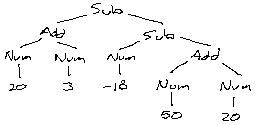
\includegraphics[width=9.4cm]{asa1.png}
          \end{center}
          \texttt{Sub( Add( Num(20) Num(3) ) Sub( Num(-18) Add( Num(50) Num(20) ) ) )}

          Semántica natural
          {\tiny
          \begin{prooftree}
            \Axi{Num(20) \Raa Num(20)} \Axi{Num(3) \Raa Num(3)}
            \BInf{Add(Num(20) Num(3)) \Raa Num(23)}
            \Axi{Num(-18) \Raa Num(-18)} 
              
              \Axi{Num(50) \Raa Num(50)} \Axi{Num(20) \Raa Num(20)}
              \BInf{Add(Num(50) Num(20)) \Raa Num(70)}

            \BInf{Sub(Num(-18) Add(Num(50) Num(20))) \Raa Num(-88)}

            \BInf{Sub(Add(Num(20) Num(3)) Sub(Num(-18) Add(Num(50) Num(20)))) \Raa Num(111)}
          \end{prooftree}
          }

          Semántica estructural
          \begin{ttt}
            Sub( Add( Num(20) Num(3) ) Sub( Num(-18) Add( Num(50) Num(20) ) ) ) \raa\\
            Sub( Num(23) Sub( Num(-18) Add( Num(50) Num(20) ) ) ) \raa\\
            Sub( Num(23) Sub( Num(-18) Num(70) ) ) \raa\\
            Sub( Num(23) Num(-88) ) \raa\\
            Num(111) \raa Num(111)
          \end{ttt}

        \item \texttt{(not (+ 1 (- 3 (+ -8 1))))}

          Sintaxis abstracta
          \begin{center}
            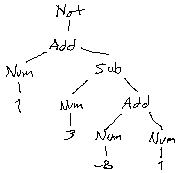
\includegraphics[width=6cm]{asa2.png}
          \end{center}
          \texttt{Not( Add( Num(1) Sub( Num(3) Add( Num(-8) Num(1) ) ) ) )}

          Semántica natural
          {\small
          \begin{prooftree}
            \Axi{Num(1) \Raa Num(1)}
              \Axi{Num(3) \Raa Num(3)}
                \Axi{Num(-8) \Raa Num(-8)}
                \Axi{Num(1) \Raa Num(1)}

                \BInf{Add(Num(-8) Num(1)) \Raa Num(-7)}
              \BInf{Sub(Num(3) Add(Num(-8) Num(1))) \Raa Num(10)}
            \BInf{Add(Num(1) Sub(Num(3) Add(Num(-8) Num(1)))) \Raa Num(11)}
            \UInf{Not(Add(Num(1) Sub(Num(3) Add(Num(-8) Num(1))))) \Raa Bool(False)}
          \end{prooftree}
          }

          Semántica estructural
          \begin{ttt}
            Not( Add( Num(1) Sub( Num(3) Add( Num(-8) Num(1) ) ) ) ) \raa\\
            Not( Add( Num(1) Sub( Num(3) Num(-7) ) ) ) \raa\\
            Not( Add( Num(1) Num(10) ) ) \raa\\
            Not( Num(11) ) \raa\\
            Bool(True) \raa Bool(True)
          \end{ttt}

        \item \texttt{(not (not (+ 3 5)))}

          Sintaxis abstracta
          \begin{center}
            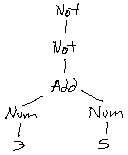
\includegraphics[width=4cm]{asa3.png}
          \end{center}
          \texttt{Not( Not( Add( Num(3) Num(5) ) ) )}

          Semántica natural
          \begin{prooftree}
            \Axi{Num(3) \Raa Num(3)}
            \Axi{Num(5) \Raa Num(5)}
            \BInf{Add( Num(3) Num(5) ) \Raa Num(8)}
            \UInf{Not( Add( Num(3) Num(5) ) ) \Raa Bool(False)}
            \UInf{Not( Not( Add( Num(3) Num(5) ) ) ) \Raa Bool(True)}
          \end{prooftree}

          Semántica estructural
          \begin{ttt}
            Not( Not( Add( Num(3) Num(5) ) ) ) \raa\\
            Not( Not( Num(8) ) ) \raa\\
            Not( Bool(False) ) \raa\\
            Bool(True) \raa Bool(True)
          \end{ttt}

      \end{enumerate}

    \item Extender la batería de operaciones de \textbf{MiniLisp}\\
      \textit{En los tres casos, deberás usar la notación formal que vimos en clase}
      \begin{itemize}
        \item Dar la gramática libre de contexto modificada (en notación EBNF) añadiendo las nuevas construcciones del lenguaje
        \item Modificar las reglas de sintaxis abstracta para considerar los nuevos constructores
        \item Extender las reglas de semántica natural y estructural 
      \end{itemize}
      \begin{enumerate}
        \item Especificar un nuevo constructor \texttt{*} para la multiplicación binaria de expresiones aritméticas. Por ejemplo
          \begin{verbatim}
> (* 20 2)
40
          \end{verbatim}

        \item Especificar un nuevo constructor \texttt{/} para la división binaria de expresiones aritméticas. Consideren que no se pueden realizar divisiones entre cero. Por ejemplo:
          \begin{verbatim}
> (/ 20 2)
10
> (/ 10 0)
error: División entre cero
          \end{verbatim}

        \item Especificar un nuevo constructor \texttt{add1} que dada una expresión, incrementa en uno su valor. Por ejemplo:
          \begin{verbatim}
> (add1 10)
11
          \end{verbatim}

        \item Especificar un nuevo constructor \texttt{sub1} que dada una expresión, decrementa en uno su valor. Por ejemplo:
          \begin{verbatim}
> (sub1 10)
9
          \end{verbatim}

        \item Especificar un nuevo constructor \texttt{sqrt} que dada una expresión, obtiene la raíz cuadrada de dicha expresión. Consideren que no se pueden calcular raíces cuadradas de números negativos. Por ejemplo:
          \begin{verbatim}
> (sqrt 81)
9
> (sqrt -2)
error: Raíz negativa
          \end{verbatim}
      \end{enumerate}

      Nueva gramática
      \begin{align*}
        &\nt{Expr} \pr \nt{Bool} \gr \nt{Num}\\
        &\qquad\qquad\quad \gr (+\ \nt{Expr}\ \ \nt{Expr})\\
        &\qquad\qquad\quad \gr (-\ \nt{Expr}\ \ \nt{Expr})\\
        &\qquad\qquad\quad \gr (*\ \nt{Expr}\ \ \nt{Expr})\\
        &\qquad\qquad\quad \gr (/\ \nt{Expr}\ \ \nt{Expr})\\
        &\qquad\qquad\quad \gr (add1 \ \nt{Expr})\\
        &\qquad\qquad\quad \gr (sub1 \ \nt{Expr})\\
        &\qquad\qquad\quad \gr (sqrt \ \nt{Expr})\\
        &\nt{Bool} \pr \#t \gr \#f\\
        &\nt{Int} \pr \nt{N} \gr -\nt{M}\\
        &\nt{D} \pr 1 \gr 2 \gr 3 \gr 4 \gr 5 \gr 6 \gr 7 \gr 7 \gr 8 \gr 9\\
        &\nt{N} \pr 0 \gr \nt{D}\{\nt{N}\}\\
        &\nt{M} \pr \nt{D}\{\nt{N}\}
      \end{align*}

      Nueva sintaxis abstracta\\
      Añadimos lo siguiente a nuesta sintaxis abstracta
      \begin{prooftree}
        \Axi{i:ASA}
        \Axi{d:ASA}
        \BInf{Mult(i, d):ASA}
      \end{prooftree}

      \begin{prooftree}
        \Axi{i:ASA}
        \Axi{d:ASA}
        \BInf{Div(i, d):ASA}
      \end{prooftree}

      \begin{prooftree}
        \Axi{c:ASA}
        \UInf{Add1(c):ASA}
      \end{prooftree}

      \begin{prooftree}
        \Axi{c:ASA}
        \UInf{Sub1(c):ASA}
      \end{prooftree}

      \begin{prooftree}
        \Axi{c:ASA}
        \UInf{Sqrt(c):ASA}
      \end{prooftree}

      Nueva semántica natural\\
      Añadimos lo siguiente a nuestra semántica natural

      \begin{prooftree}
        \Axi{i \Raa Num(i')}
        \Axi{d \Raa Num(d')}
        \BInf{Mult(i, d) \Raa Num(i' * d')}
      \end{prooftree}

      \begin{prooftree}
        \Axi{i \Raa Num(i')}
        \Axi{d \Raa Num(0)}
        \BInf{Div(i, d) \Raa error: División entre 0}
      \end{prooftree}

      \begin{prooftree}
        \Axi{i \Raa Num(i')}
        \Axi{d \Raa Num(d')}
        \BInf{Div(i, d) \Raa Num(i' / d')}
      \end{prooftree}

      \begin{prooftree}
        \Axi{c \Raa Num(c')}
        \UInf{Add1(c) \Raa Num(c' + 1)}
      \end{prooftree}

      \begin{prooftree}
        \Axi{c \Raa Num(c')}
        \UInf{Sub1(c) \Raa Num(c' - 1)}
      \end{prooftree}

      \begin{prooftree}
        \Axi{c \Raa Num(c')}
        \Axi{c' < 0}
        \BInf{Sqrt(c) \Raa error: Raíz negativa}
      \end{prooftree}

      \begin{prooftree}
        \Axi{c \Raa Num(c')}
        \UInf{Sqrt(c) \Raa Num($\sqrt{\text{c'}}$)}
      \end{prooftree}

      Nueva semántica estructural\\
      Añadimos lo siguiente a nuestra semántica estructural

      \begin{prooftree}
        \Axi{i \raa i'}
        \UInf{Mult(i, d) \raa Mult(i', d)}
      \end{prooftree}

      \begin{prooftree}
        \Axi{d \raa d'}
        \UInf{Mult(Num(i), d) \raa Mult(Num(i), d')}
      \end{prooftree}

      \begin{prooftree}
        \Axi{-}
        \UInf{Mult(Num(i), Num(d)) \raa Num(i * d)}
      \end{prooftree}

      \begin{prooftree}
        \Axi{i \raa i'}
        \UInf{Div(i, d) \raa Div(i', d)}
      \end{prooftree}

      \begin{prooftree}
        \Axi{d \raa d'}
        \UInf{Div(Num(i), d) \raa Div(Num(i), d')}
      \end{prooftree}

      \begin{prooftree}
        \Axi{-}
        \UInf{Div(Num(i), Num(0)) \raa error: División entre 0}
      \end{prooftree}

      \begin{prooftree}
        \Axi{-}
        \UInf{Div(Num(i), Num(d)) \raa Num(i / d)}
      \end{prooftree}

      \begin{prooftree}
        \Axi{c \raa c'}
        \UInf{Add1(c) \raa Add1(c')}
      \end{prooftree}

      \begin{prooftree}
        \Axi{-}
        \UInf{Add1(Num(c)) \raa Num(c + 1)}
      \end{prooftree}

      \begin{prooftree}
        \Axi{c \raa c'}
        \UInf{Sub1(c) \raa Sub1(c')}
      \end{prooftree}

      \begin{prooftree}
        \Axi{-}
        \UInf{Sub1(Num(c)) \raa Num(c - 1)}
      \end{prooftree}

      \begin{prooftree}
        \Axi{c \raa c'}
        \UInf{Sqrt(c) \raa Sqrt(c')}
      \end{prooftree}

      \begin{prooftree}
        \Axi{c < 0}
        \UInf{Sqrt(Num(c)) \raa error: Raíz negativa}
      \end{prooftree}

      \begin{prooftree}
        \Axi{-}
        \UInf{Sqrt(Num(c)) \raa Num($\sqrt{\text{c}}$)}
      \end{prooftree}

  \end{enumerate}
\end{document}
